\documentclass{article}%
\usepackage[T1]{fontenc}%
\usepackage[utf8]{inputenc}%
\usepackage{lmodern}%
\usepackage{textcomp}%
\usepackage{lastpage}%
\usepackage{authblk}%
\usepackage{graphicx}%
%
\title{Neurogenesis and Increase in Differentiated Neural Cell Survival via Phosphorylation of Akt1 after Fluoxetine Treatment of Stem Cells}%
\author{Sean Alvarado}%
\affil{Division of Infection and Immunity, University College London, London, United Kingdom}%
\date{01{-}01{-}2011}%
%
\begin{document}%
\normalsize%
\maketitle%
\section{Abstract}%
\label{sec:Abstract}%
SAN DIEGO, CA (LINK\_1544174) {-} Piaries Research Institute at UC San Diego is exploring the potential of catalyzing the PI3K/AKT/NFkB pathway as a model for population oncology for patients with COPD and other progressive lung diseases. Researchers believe their model could enhance our understanding of cancer development and neurocognitive outcomes from such diseases as Parkinsons, Alzheimers and multiple sclerosis.\newline%
They discovered that broadities of APL{-}D, MPL{-}CRS, TIR{-}PD, SODIC{-}V, TULAN, and NRH{-}OCL1 gene expression prior to chemotherapy in lung cancer cells activate PI3K kinase mutations, activating the multi{-}polar kinase pathway that led to these cells becoming idle and eventually turning into cancer cells. In addition, the peak expression of PI3K/AKT/NFkB in vivo enhanced the progression of cancer.\newline%
These findings may explain why ALL patients with aggressive lung diseases have had significant response rates to prior chemotherapy, while many with milder forms of COPD do not, said said Robert A. Pait, PhD, a research associate at UC San Diego. These findings could also generate opportunities for biomarkers that predict lung cancer survival in order to predict the course of disease in a patient.\newline%
The research team is completing a translational study involving rats, a clinical cohort of lung cancer patients, and other lung malignancies to investigate the potential of inhibiting PI3K/AKT/NFkB throughactivation through the PI3K/AKT pathway.\newline%
Pait and his colleagues have also strengthened their models for the PI3K/AKT/NFkB pathway, focusing specifically on the ability of PI3K/AKT to inhibit or inhibit a particular cell line protein (TLP2). Such cellular signaling play an important role in regulating cellular responses to tumor development and cancer cell disease, and it is the strong signaling mechanisms associated with CYP2c, the implicated T{-}DM1{-}like protein, that make PI3K/AKT/NFkB function so important for tumor growth.\newline%
The study results were published in The Journal of Cell Biology.\newline%
The PI3K/AKT/NFkB pathway is implicated in many clinical and translational diseases. This pathway can be used as a model for a variety of diseases, including CNS (nervous, parietal, gastrointestinal, aminobiochemistry, and amyloid plaques) from lung, as well as cancer in human species from the classical cell divide to the NSCLC (prostate, liver, colon, gastric, kidney, and bladder cancer) proliferative cellular life cycle. The pathway is also used in humans to generate beta{-}cells in the developing nervous system to produce therapeutics to treat neurological conditions.

%
\subsection{Image Analysis}%
\label{subsec:ImageAnalysis}%


\begin{figure}[h!]%
\centering%
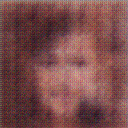
\includegraphics[width=150px]{500_fake_images/samples_5_226.png}%
\caption{A Close Up Of A Mirror On A Wall}%
\end{figure}

%
\end{document}